\documentclass[12pt, fleqn]{article}

\makeatletter
\renewcommand*\l@section{\@dottedtocline{1}{1.5em}{2.3em}}



%\includegraphics{universe}

\usepackage[utf8]{inputenc}
\usepackage[T2A]{fontenc}
\usepackage[russian]{babel} % указывает язык документа
\usepackage[left=2cm,right=2cm,top=2cm,bottom=2cm,bindingoffset=0cm]{geometry}
\usepackage{lastpage}
\usepackage{fancyhdr}
\usepackage[uppercase]{titlesec}
\usepackage{graphicx} % для вставки картинок
\usepackage{mathtools, amssymb} % математические дополнения
\usepackage[tableposition=top]{caption}
\usepackage{subcaption}
\usepackage{indentfirst}
\usepackage{pythonhighlight}
\usepackage{listings}
\usepackage{tabularx}
\usepackage{tabulary}
\usepackage{float}
\usepackage[figure,table]{totalcount}
\usepackage{diagbox}

\usepackage{hyperref}

\setlength{\parindent}{1em}

%\setlength{\section*}{0.5cm}
%\usepackage{minted}
%\usepackage{fancyvrb}
%\usepackage{mathptmx}% http://ctan.org/pkg/mathptmx
%\usepackage{newtxtext}

%\titleformat{\section}[hang]{\bfseries\LARGE\centering}{}{1em}{}
\titleformat*{\section}{\large\bfseries\centering}
\titleformat{\subsection}[block]{\bfseries\hspace{1em}}{\thesubsection}{0.5em}{}
%\setlength{\subsection*}{1.5cm}
%\setlength{\parindent}{4em}

%\setlength{\parindent}{1.5cm}

\captionsetup[figure]{labelfont={it},textfont={it},name={Рисунок},labelsep=endash, skip=5pt}
\captionsetup[table]{labelfont={it},textfont={it},name={Таблица},labelsep=endash,singlelinecheck=false, skip=5pt, margin=1cm}


\linespread{1.3} % полуторный интервал
\frenchspacing
\graphicspath{ {images/} }

  %-------------------------------------------
  % Переменные
  %-------------------------------------------

  \newcommand{\authorSurName}{Белоусов} % Фамилия автора
  \newcommand{\authorInitials}{ А.А.} % Фамилия автора
  \newcommand{\variantNumber}{51} % Номер варианта
  \newcommand{\recordBookNumber}{146166} % Номер зачетной книжки
  \newcommand{\groupNumber}{6309} %Номер группы
 
  %-------------------------------------------
  % Ссылки в оглавлении
  %-------------------------------------------
  

\hypersetup{
    colorlinks,
    citecolor=black,
    filecolor=black,
    linkcolor=black,
    urlcolor=black
}

  %-------------------------------------------
  % Стиль футеров и хедеров
  %-------------------------------------------

\pagestyle{fancy}
\fancyhead[L, R]{}
\fancyfoot[L]{Случайные процессы АРСС}
\fancyfoot[R]{\groupNumber-\authorSurName-\variantNumber}
\renewcommand{\footrulewidth}{0pt}
\renewcommand{\headrulewidth}{0pt}

%\renewcommand\subsectionfont{\normalfont\normalsize\bfseries}

\def\l@subsection{\@dottedtocline{2}{3.8em}{3.2em}}

% Для листинга

\lstset{
basicstyle=\footnotesize\ttfamily,
columns=fullflexible,
keywordstyle=\color{blue},
%frame=single,
breaklines=true,
numberstyle=\tiny\color{mygray},
postbreak=\mbox{\textcolor{red}{$\hookrightarrow$}\space},
showstringspaces=false,
}

\newcolumntype{Y}{>{\centering\arraybackslash}X}

\begin{document}

%----------------------------------------------------------------------------------------
%	TITLE PAGE
%----------------------------------------------------------------------------------------
\pagenumbering{Alph}

\begin{titlepage}
							
	\center
							
	%------------------------------------------------
	%	Заголовки
	%------------------------------------------------
							
	\textsc{\textbf{МИНИСТЕРСТВО ОБРАЗОВАНИЯ И НАУКИ РОССИЙСКОЙ ФЕДЕРАЦИИ}}\\[0.1cm]
	\textsc{\small\textbf{Федеральное государственное автономное образовательное учреждение высшего образования}}\\[0.05cm] 
	\textsc{\small\textbf{«Самарский национальный исследовательский университет
		имени академика С.П.Королёва»}}\\[0.05cm] 
	\textsc{\textit{ИНСТИТУТ ИНФОРМАТИКИ, МАТМАТИКИ И ЭЛЕКТРОНИКИ}}\\[0.2cm]
	\textsc{\textit{ФАКУЛЬТЕТ ИНФОРМАТИКИ}}\\[0.1cm]
	\textsc{\textit{КАФЕДРА ТЕХНИЧЕСКОЙ КИБЕРНЕТИКИ}}\\[0.5cm]
						
	%------------------------------------------------
	%	Название работы
	%------------------------------------------------
							
	\vfill\vfill
						    
							
	{\large СТАТИСТИЧЕСКИЙ АНАЛИЗ И МОДЕЛИРОВАНИЕ ПРОЦЕССОВ АВТОРЕГРЕССИИ И СКОЛЬЗЯЩЕГО СРЕДНЕГО}\\[0.3cm]
	{\large курсовая работа по дисциплине «\textbf{Теория случайных процессов}»}\\[0.5cm]
	{\centering\large Вариант № \variantNumber}\\[1.5cm]
						  
	\vfill\vfill\vfill
							
	\begin{minipage}{1\textwidth}
		\begin{flushright}
			\begin{tabular}{l l}
				Выполнил:                  & \authorSurName \authorInitials \\
				Группа:                      & 6309                           \\
				№ зачетной книжки: & \recordBookNumber              \\
				Проверил:                  & Храмов  А. Г.          \\
				Оценка:                      & $\rule{3cm}{0.15mm}$           \\
				Дата:                          & $\rule{3cm}{0.15mm}$           
			\end{tabular}
		\end{flushright}
	\end{minipage}
							
						
	%------------------------------------------------
	%	Дата
	%------------------------------------------------
							
	\vfill\vfill\vfill
					
	{\centering Самара 2018}
							
							
\end{titlepage}
\pagenumbering{arabic}
\setcounter{page}{2}
%------------------------------------------------
%Реферат
%------------------------------------------------
\newpage
\section*{Реферат}
{
	\textbf{Курсовая работа по курсу «Теория случайных процессов»} 
	\pageref{LastPage} страниц,
	\totalfigures\ рисунков,
	\totaltables\ таблиц,
	3 источника,
	2 приложения.\\
				
	МОМЕНТНЫЕ ФУНКЦИИ, МАТЕМАТИЧЕСКОЕ ОЖИДАНИЕ, ДИСПЕРСИЯ, КОРРЕЛЯЦИОННАЯ ФУНКЦИЯ, МОДЕЛЬ АВТОРЕГРЕСИИ, МОДЕЛЬ СКОЛЬЗЯЩЕГО СРЕДНЕГО, МОДЕЛЬ ARMA\\
						  
	Объектом исследований является выборка из $n = 5000$ последовательных значений стационарного в широком смысле эргодичного случайного процесса с дискретным временем (временной ряд).
						  
	Цель работы -- оценка моментных функций, построение и исследование моделей авторегрессии, скользящего среднего, смешанных моделей, моделирование случайных процессов.
						  
	Были расчитаны выборочные моментные функции, построены и исследованы модели АР, СС, АРСС. Проведено моделирование процессов АР(3), СС(1), АРСС(3, 1).
}

%----------------------------------------------------------------------------------------

%------------------------------------------------
%	Содержание
%------------------------------------------------

\newpage
\tableofcontents
\newpage
%----------------------------------------------------------------------------------------


%--------------------------------------------
% Задание
%--------------------------------------------
\newpage
\section{Задание}

{
							
	\subsection{Оценивание моментных функций}{
		Изобразить графически фрагмент исходного случайного процесса (СП). Оценить моментные функции (МФ) исходного случайного процесса, рассчитав выборочные среднее, дисперсию и нормированную корреляционную функцию (НКФ). Оценить интервал корреляции СП. Изобразить графически оценку НКФ исходного СП.
	}
	\subsection{Построение и исследование моделей авторегрессии}
	{
		Построить модели авторегрессии АР(M) = АРСС(M, 0) порядков M = 0, 1, 2, 3 (всего 4
		модели) на основе решения системы уравнений Юла–Уокера. Для каждой модели рассчитать
		теоретические НКФ выходной последовательности. На основе сравнения выборочной НКФ и
		теоретических НКФ выбрать лучшую модель СП в классе моделей АР.
	}
							
	\subsection{Построение и исследование моделей скользящего среднего}
	{
		Построить модели скользящего среднего СС(N) = АРСС(0, N) порядков N = 0, 1, 2, 3
		(всего 4 модели) на основе решения системы нелинейных уравнений. Для каждой модели
		рассчитать теоретические НКФ выходной последовательности. На основе сравнения выбо-
		рочной НКФ и теоретических НКФ выбрать лучшую модель СП в классе моделей СС.
	}
							
	\subsection{Построение и исследование смешанных моделей авторегрессии – скользящего среднего}
	{
		Построить смешанные модели авторегрессии – скользящего среднего АРСС(M, N) до
		третьего порядка включительно (M = 1, 2, 3; N = 1, 2, 3) (всего 9 моделей) одним из методов,
		описанным в приложении А.3. Рассчитать теоретические НКФ выходной последовательности
		для каждой модели АРСС. На основе сравнения исходной выборочной и теоретических НКФ
		выбрать лучшую модель СП в классе смешанных моделей АРСС. Исследовать на устойчи-
		вость смешанные модели.
	}
							
	\subsection{Сравнительный анализ построенных моделей}
	{
		Для каждой из трёх лучших моделей (АР, СС, АРСС) записать системы уравнений для
		расчёта параметров модели, записать системы уравнений для расчёта теоретической КФ,
		смоделировать СП, рассчитать выборочные МФ, сравнить их с выборочными МФ исходного
		СП и с теоретическими МФ. Для каждой из этих трёх моделей сравнить графически НКФ:
		(1) выборочную исходного СП, (2) теоретическую, (3) выборочную смоделированного СП.
	}
							
	\subsection{Итоговая таблица сравнения моделей АРСС}{
		Изготовить таблицу сравнения МФ и расчёта качества для трёх лучших моделей. Изоб-
		разить графически фрагмент реализации СП, сгенерированного по наилучшей модели.
	}
}

%-----------------------------------------------
% Исходные данные.  %-----------------------------------------------
\newpage
\section{Исходные данные}
  
{
	Дана реализация стационарного в широком смысле эргодического случайного процесса с дискретным временем (стационарная случайная последовательность, временной ряд) – выборка из $n = 5000$ последовательных значений (отсчётов) процесса:\\
						  
-26.364 -31.116 -16.294 -33.269 -12.440 -36.868 -21.972 -29.761 -14.903 -33.905 -13.594 -37.352 -20.000 -32.988 -13.362 -23.077 -14.026 -23.744 -31.442 -39.546 -36.071 -20.985 -21.972 -23.090 -25.598 -20.838 -21.724 -21.249 -27.790 -23.872 -27.504 -27.615 -29.436 -31.517 -17.928

...

-29.333 -23.756 -16.822 -27.577 -20.445 -17.546 -30.783 -18.043 -33.864 -18.692 -35.802 -15.114 -36.468 -17.033 -41.076 -14.229 -36.877 -18.515 -36.372 -10.348 -28.443 -13.548 -38.428 -21.716 -37.438 -13.258 -33.314 -7.763 -33.864 -15.854 -35.060 -24.056 -29.442 -21.433 -25.555

		
						  
}


%--------------------------------------------------
% Оценивание моментных функций
%--------------------------------------------------
\newpage
\section{Оценивание моментных функций}
{
	\subsection{Графическое представление}
	Графически изобразим фрагмент исходного случайного процесса на рисунке 1.
	\begin{figure}[H]
		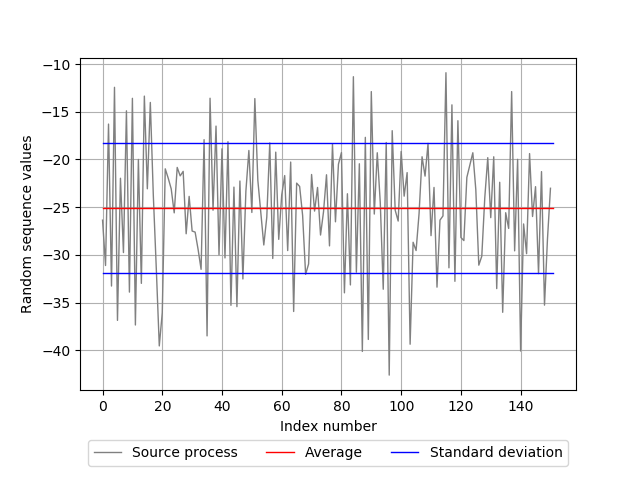
\includegraphics{plot1.png}
		\caption{График исходного случайного процесса}
	\end{figure}
						    
	\subsection{Моментные функции}
	Пусть дана выборка $X_{1} ... X_{n}$ из $n$ отсчётов стационарного в широком смысле эргодического дискретного случайного процесса. Оценим моментные функции этого процесса, рассчитав:
	\begin{enumerate}
		\item Выборочное среднее
		\item Выборочную дисперсию
		\item Нормированную корреляционную функцию (НКФ).
	\end{enumerate}
						      
	\begin{enumerate}
		\item {
			Выборочное среднее $\overline{X}$ - это оценка математического ожидания $\mathbb{M}(X)$. Формула для расчётов:
			\begin{equation}
				\overline{X}=\frac{1}{n}\sum_{k=1}^{n} X_k,
			\end{equation}
			где $X_k$ - элементы выборки при $k \in [0, n]$, а $n$ - размер выборки.        
																		        
			Используя программу из приложения А, получаем $\overline{X} = -25.072198200000003$.
																		        
			На рисунке 1 показано значение $ \overline{X} $.
		}
		\item
		      {
		      	Выборочная дисперсия $S^2$ - это оценка дисперсии $D(\overline{X})=D_x$ распределения на основе выборки.
		      	Различают два вида дисперсии -- выборочную и несмещённую.
		      			      			      			      			      			      	        
		      	Формула для расчёта выборочной дисперсии:
		      	\begin{equation}
		      		{S^2}_n=\frac{1}{n}\sum_{k=1}^{n}{(X_k - \overline{X})^2}.
		      	\end{equation}
		      			      			      			      			      			      	        
		      	Формула для расчёта несмещённой или исправленной дисперсии:
		      	\begin{equation}\label{disp}
		      		{\hat{S}^2}_n=\frac{1}{n-1}\sum_{k=1}^{n}{(X_k - \overline{X})^2}.
		      	\end{equation}
		      			      			      			      			      			      	        
		      	В данном случае была использована исправленная дисперсия, т.к. она даёт несмещённую оценку дисперсии:
		      	\begin{equation}
		      		M({\hat{S}^2}_n)=D_x.
		      	\end{equation}
		      			      			      			      			      			      	        
		      	Применяя формулу \eqref{disp}, получаем $\hat{S}^2_n = 45.94676292851676$.
		      			      			      			      			      			      	        
		      	Для вычисления среднеквадратического отклонения (СКО) используется следующая формула:
		      	\begin{equation}
		      		\hat{S}_n=\sqrt{\frac{1}{n-1}\sum_{k=1}^{n}{(X_k - \overline{X})^2}}.
		      	\end{equation}
		      			      			      			      			      			      	        
		      	Принимая во внимание значение $ \hat{S}^2_n $, получаем $ \hat{S}_n = 6.778404157950215 $.
		      			      			      			      			      			      	        
		      	На рисунке 1 отображены значения $ \overline{X} + \hat{S}_n $ и $ \overline{X} - \hat{S}_n $.
		      }
		\item
		      {
		      	Формула для вычисления оценки исправленой выборочной корреляционной функции $ \hat{R}_\xi(k) $:		      			      			      			      		  	
		      	\begin{equation}\label{corr_func}
		      		\hat{R}_\xi(k) = \frac{1}{n - k - 1} \sum_{j=1}^{n - k} {(X_j - \overline{X})(X_{j+k}-\overline{X})}.
		      	\end{equation}
		      			      			      			      			      			      		  	
		      	В таблице 1 представлены значения этой функции для $ k = 0,1,\dots10 $.
		      			      			      			      			      			      		  	
		      	Оценка нормированной корреляционной функции $ \hat{r}_\xi(k) $ определяется следующим образом:
		      	\begin{equation}
		      		\hat{r}_\xi(k) = \frac{\hat{R}_\xi(k)}{\hat{R}_\xi(0)} = \frac{\hat{R}_\xi(k)}{\hat{S}^2_n}.
		      	\end{equation}
		      			      			      			      			      			      		  	
		      	Её значения для $ k = 0,1,\dots10 $ также представлены в таблице 1.
		      	\begin{table}[H]
		      		\centering
		      		\caption{Значения выборочных КФ и НКФ}
		      		\begin{tabularx}{0.9\textwidth}{ |Y|Y|Y| }
		      			\hline
		      			k  & $ \hat{R}_\xi(k) $ & $ \hat{r}_\xi(k) $ \\ \hline
		      			0  &  45.94676 &  1.0      \\ \hline
					1  &  -16.83377 &  -0.36638      \\ \hline
					2  &  20.06587 &  0.43672      \\ \hline
					3  &  -20.94726 &  -0.4559      \\ \hline
					4  &  11.22639 &  0.24433      \\ \hline
					5  &  -14.17409 &  -0.30849      \\ \hline
					6  &  8.02627 &  0.17469      \\ \hline
					7  &  -8.94403 &  -0.19466      \\ \hline
					8  &  5.63892 &  0.12273      \\ \hline
					9  &  -5.55074 &  -0.12081      \\ \hline
					10  &  3.49849 &  0.07614      \\ \hline
		      		\end{tabularx}
		      	\end{table}
		      			      			      			      	
		      	Оценим интервал корреляции:
		      	\begin{equation}
		      		\tau_\text{к} = min \{\tau : \forall(m > \tau) \left|r_\eta(m) \right| < \frac{1}{e} \},
		      	\end{equation}
		      	полагая что $ m << n $.
		      			      			      			      			      			      	  
		      	Используя программу из проложения А, получаем значение $ \tau_\text{к}  = 3 $. На рисунке 2 изображена оценка интервала корреляции исходного случайного процесса.
		      	\begin{figure}[H]
		      		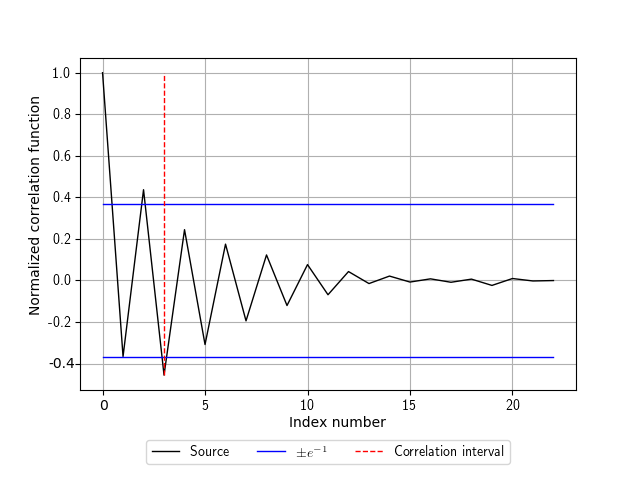
\includegraphics{plot2.png}
		      		\caption{Графическая оценка интервала корреляции}
		      	\end{figure}
		      }
	\end{enumerate}
}
  

%--------------------------------------------------
% Построение и исследование моделей авторегрессии
%--------------------------------------------------
\newpage
\section{Построение и исследование моделей авторегрессии}
{
	\subsection{Модель АРСС($M$, $0$)}
	{
		Модель авторегрессии порядка $M$ в общем виде может быть записанна как:
		\begin{equation}
			\eta_n = \beta_1\eta_{n-1} + \beta_2 \eta_{n-2} + \dots + \beta_M \eta_{n-M} +\alpha_0 \xi_n,
		\end{equation}
		где $\xi$ -- входная некоррелированная случайная последовательность с нулевым математическим ожиданием и единичной дисперсией ($\mathbb{M}(\xi_n)=0$, $\mathbb{M}(\xi^2_n)=1$, $\mathbb{M}(\xi_k \xi_n)=\delta_{kn}$), $\eta$ -- выходная случайная, стационарная в широком смысле последовательность с корреляционной функцией $R_{\eta}(m)$ и нулевым математическим ожиданием, $\{M, \alpha_0, \beta_1, \beta_2, \dots, \beta_M\}$ -- параметры модели авторегрессии.\medskip 
										      
		Построим модели авторегрессии для $M = 0,1,2,3$ на основе решения системы уравнений Юла-Уокреа. Для решения линейных систем был использован метод numpy.linalg.solve из библиотеки numpy. Выпишем системы уравнений.\medskip 
										      
		Для модели АРСС(0, 0) получаем:
		\begin{equation}\label{ar0}
			R_{\eta}(0) = \alpha^2_0
		\end{equation}
		Решая уравнение \eqref{ar0}, получаем $\alpha_0 = 6.77840416$.\medskip 
										      
		Для модели АРСС(1, 0) получаем:
		\begin{equation}\label{ar1}
			\left\{
			\begin{split}
				R_{\eta}(0) &= \beta_1 R_{\eta}(1) + \alpha^2_0 \\
				R_{\eta}(1) &= \beta_1 R_{\eta}(0)
			\end{split}
			\right.
		\end{equation}
		Решая систему \eqref{ar1}, получаем $\alpha_0 = 6.30708201$, $\beta_1 = -0.36637548$.\medskip 
										      
		Для модели АРСС(2, 0) получаем:
		\begin{equation}\label{ar2}
			\left\{
			\begin{split}
				R_{\eta}(0) &= \beta_1 R_{\eta}(1) + \beta_2 R_{\eta}(2) + \alpha^2_0 \\
				R_{\eta}(1) &= \beta_1 R_{\eta}(0) + \beta_2 R_{\eta}(1) \\
				R_{\eta}(2) &= \beta_1 R_{\eta}(1) + \beta_2 R_{\eta}(0)
			\end{split}
			\right.
		\end{equation}
		Решая систему \eqref{ar2}, получаем $\alpha_0 = 5.90959855$, $\beta_1 = -0.23836838$, $\beta_2 = 0.34938774$.\medskip 
										      
		Для модели АРСС(3, 0) получаем:
		\begin{equation}\label{ar3}
			\left\{
			\begin{split}
				R_{\eta}(0) &= \beta_1 R_{\eta}(1) + \beta_2 R_{\eta}(2) + \beta_3 R_{\eta}(3) + \alpha^2_0 \\
				R_{\eta}(1) &= \beta_1 R_{\eta}(0) + \beta_2 R_{\eta}(1) + \beta_3 R_{\eta}(2) \\
				R_{\eta}(2) &= \beta_1 R_{\eta}(1) + \beta_2 R_{\eta}(0) + \beta_3 R_{\eta}(1) \\
				R_{\eta}(3) &= \beta_1 R_{\eta}(2) + \beta_2 R_{\eta}(1) + \beta_3 R_{\eta}(0)
			\end{split}
			\right.
		\end{equation}
		Решая систему \eqref{ar3}, получаем $\alpha_0 = 5.64763391$, $\beta_1 = -0.1354962$, $\beta_2 = 0.27920361$, $\beta_3 = -0.29443558$.\medskip 
										      
		Проверим полученные модели на устойчивость. Для этого выясним лежат ли все корни $z$ характерестического уравнения \eqref{chareq} внутри единичной окружности $ \left| z \right| < 1 $ на комплексной плоскости:
		\begin{equation}\label{chareq}
			\sum_{k=1}^M {\beta_k z^{-k}} = 1.
		\end{equation}\medskip 
										      

		Рассмотрим каждую модель:
		\begin{itemize}
			\item {
				Модель АРСС(0, 0) устойчива всегда.
			}
			\item {
				Модель АРСС(1, 0) устойчива тогда и только тогда, когда $\left| \beta_1 \right| < 1$:
				\begin{equation*}
					\left|  -0.36637548 \right| < 1 \Rightarrow \text{Модель устойчива}.
				\end{equation*}
			}
			\item {
				Модель АРСС(2, 0) устойчива тогда и только тогда, когда $\left| \beta_2 \right| < 1$, $\left| \beta_1 \right| < 1 - \beta_2$:
				\begin{equation*}
					\left.
					\begin{split}
						&\left| 0.34938774 \right| < 1 \\
						&\left| -0.23836838 \right| < 0.65061226
					\end{split}
					\right\} \Rightarrow \text{Модель устойчива}.
				\end{equation*}
			}
			\item {		% Остановился тут
				Модель АРСС(3, 0) устойчива тогда и только тогда, когда $\left| \beta_3 \right| < 1$, $\left| \beta_1 + \beta_3 \right| < 1 - \beta_2$, $\left| \beta_2 + \beta_1 \beta_3 \right| < \left| 1 - \beta^2_3 \right|$:
				\begin{equation*}
					\left.
					\begin{split}
						&\left| -0.29443558 \right| < 1 \\
						&\left| -0.42993178 \right| < 0.72079639 \\
						&\left|  0.31909851 \right| < 0.08669231
					\end{split}
					\right\} \Rightarrow \text{Модель устойчива}.
				\end{equation*}
			}
		\end{itemize}
	}
					
	\subsection{Расчёт теоретической НКФ выходной последовательности} {
		Для каждой модели рассчитаем теоретическую НКФ выходной последовательности. Для этого воспользуемся следующей формулой:
		\begin{equation}
			r_{\eta}^{\text{Т}}(M + k) = \sum_{j=1}^{M}{b_j r_{\eta}^{\text{Т}}(M + k - j)}, k \geq 1,
		\end{equation}
		учитывая что первые $M + 1$ значений теоретической НКФ нам уже известны, т.к. они совпадают с первыми значениями выборочной НКФ для исходных данных. \medskip
				
		Полученные значения, для $k = 0,1,2,\dots,10$, представлены в таблице 2.
		\begin{table}[H]\label{tbl_ncf_ar}
			\centering
			\caption{Значения теоретических НКФ для моделей АР(M)}
			\begin{tabularx}{0.9\textwidth}{ |Y|Y|Y|Y|Y| }
				\hline
				$r_{\eta}^{\text{Т}}(k)$  & АР(0) & АР(1) & АР(2)  & АР(3)  \\ \hline
				$r_{\eta}^{\text{Т}}(0)$  & 1.00000 & 1.00000 & 1.00000  & 1.00000  \\ \hline
				$r_{\eta}^{\text{Т}}(1)$  & 0.00000 & 0.36654 & 0.36654  & 0.36654  \\ \hline
				$r_{\eta}^{\text{Т}}(2)$  & 0.00000 & 0.13435 & -0.20896 & -0.20896 \\ \hline
				$r_{\eta}^{\text{Т}}(3)$  & 0.00000 & 0.04925 & -0.25234 & -0.84118 \\ \hline
				$r_{\eta}^{\text{Т}}(4)$  & 0.00000 & 0.01805 & -0.0463  & -0.46067 \\ \hline
				$r_{\eta}^{\text{Т}}(5)$  & 0.00000 & 0.00662 & 0.07637  & 0.06634  \\ \hline
				$r_{\eta}^{\text{Т}}(6)$  & 0.00000 & 0.00243 & 0.05746  & 0.68406  \\ \hline
				$r_{\eta}^{\text{Т}}(7)$  & 0.00000 & 0.00089 & -0.00087 & 0.50414  \\ \hline
				$r_{\eta}^{\text{Т}}(8)$  & 0.00000 & 0.00033 & -0.02324 & 0.0545   \\ \hline
				$r_{\eta}^{\text{Т}}(9)$  & 0.00000 & 0.00012 & -0.01155 & -0.53334 \\ \hline
				$r_{\eta}^{\text{Т}}(10)$ & 0.00000 & 0.00004 & 0.0033   & -0.50832 \\ \hline
			\end{tabularx}
		\end{table}
									
		\subsection{Выбор налучшей модели случайного процесса в классе моделей АР} {
			Выбор лучшей модели проводится на основе анализа нормированных корреляционных функций с использованием критерия среднего квадратичного отклонения по первым десяти отсчётам:
			\begin{equation}\label{best_criterion}
				\epsilon^2 = \sum_{k=1}^{10} {(r^{\text{Т}}(k) - \hat{r}(k))^2},
			\end{equation}
		}
		где $\hat{r}(k)$ -- выборочная НКФ исходного процесса, $r^{\text{Т}}$ -- теоретическая НКФ.
		Результаты представлены в таблице 3. По результатам делаем следующий вывод: среди данных моделей, процесс лучше всего описывает модель АР(3).
		\begin{table}[H]
			\centering
			\caption{Результаты построения моделей АР(М)}
			\begin{tabularx}{0.95\textwidth}{ | Y | Y | Y | Y | Y | Y | }
				\hline
				Порядок модели & \multicolumn{4}{c|}{Параметры модели} & Погрешность модели \\ \hline
				$M$ & $\beta_1$ & $\beta_2$ & $\beta_3$ & $\alpha_0$ & $\epsilon^2$ \\ \hline
				0   & -         & -         & -         & 15.76559   & 2.37896      \\ \hline
				1   & 0.36654   & -         & -         & 14.66832   & 2.41631      \\ \hline
				2   & 0.51191   & -0.39660  & -         & 13.46541   & 1.71611      \\ \hline
				3   & 0.19178   & 0.01662   & -0.80719  & 7.94843    & 0.00011      \\ \hline
			\end{tabularx}
		\end{table}
									
	}
				
	%--------------------------------------------------
	% Построение и исследование моделей скользящего среднего
	%--------------------------------------------------
	\newpage
	\section{Построение и исследование моделей скользящего среднего}
	{
		\subsection{Модель АРСС($0$, $N$)} {
			Модель скользящего среднего порядка $N$ в общем виде может быть записана как:
			\begin{equation}
				\eta_n = \alpha_0 \xi_n + \alpha_1 \xi_{n-1} + \dots + \alpha_N \xi_{n - N},
			\end{equation}
			где $\xi$ -- входная некоррелированная случайная последовательность с нулевым математическим ожиданием и единичной дисперсией ($\mathbb{M}(\xi_n)=0$, $\mathbb{M}(\xi^2_n)=1$, $\mathbb{M}(\xi_k \xi_n)=\delta_{kn}$), $\eta$ -- выходная случайная, стационарная в широком смысле последовательность с корреляционной функцией $R_{\eta}(m)$ и нулевым математическим ожиданием, $\{N, \alpha_0, \alpha_1, \alpha_2, \dots, \alpha_N\}$ -- параметры модели скользящего среднего.\medskip
								  
			Построим модели скользящего среднего для $N = 0,1,2,3$ на основе решения системы нелинейных уравнений. Решение будем получать исходя из известных значений выборочной корреляционной функции $R_{\eta}(m)$ и следующей системы нелинейных уравнений:
			\begin{equation}
				R_{\eta}(m) = 
				\begin{cases}
					\displaystyle\sum_{n=1}^{N-m}{\alpha_n \alpha_{n+M}} & \text{если } m \leq N \\
					0                                                    & \text{иначе}         
				\end{cases}
			\end{equation}
								  
			Выпишем системы для СС(0), СС(1), СС(2) и СС(3). Решим эти системы используя метод простых итераций из приложения Б.
								  
			\begin{itemize}
				\item {
					Для СС(0) получаем:
					\begin{equation*}
						R_{\eta}(0) = \alpha_0^2 \rightarrow \alpha_0^2 = 248.55388 \rightarrow \alpha_0 = 15.76559.
					\end{equation*}
				}
				\item {
					Для СС(1) получаем:
					\begin{equation*}
						\left\{
						\begin{split}
							R_{\eta}(0) &= \alpha_0^2 + \alpha_1^2 \\
							R_{\eta}(1) &= \alpha_0 \alpha_1
						\end{split}
						\right. \rightarrow \alpha_0 = 14.44998, \alpha_1 = 6.30492.
					\end{equation*}
				}
				\item {
					Для СС(2) получаем:
					\begin{equation*}
						\left\{
						\begin{split}
							R_{\eta}(0) &= \alpha_0^2 + \alpha_1^2 + \alpha_2^2 \\
							R_{\eta}(1) &= \alpha_0 \alpha_1 + \alpha_1 \alpha_2 \\
							R_{\eta}(2) &= \alpha_0 \alpha_2
						\end{split}
						\right. \rightarrow \text{Система не имеет решения}.
					\end{equation*}
				}
				\item {
					Для СС(3) получаем:
					\begin{equation*}
						\left\{
						\begin{split}
							R_{\eta}(0) &= \alpha_0^2 + \alpha_1^2 + \alpha_2^2 + \alpha_3^2 \\
							R_{\eta}(1) &= \alpha_0 \alpha_1 + \alpha_1 \alpha_2 + \alpha_2 \alpha_3 \\
							R_{\eta}(2) &= \alpha_0 \alpha_2 + \alpha_1 \alpha_3 \\
							R_{\eta}(3) &= \alpha_0 \alpha_3
						\end{split}
						\right. \rightarrow \text{Система не имеет решения}.
					\end{equation*}
				}				
			\end{itemize}
						
			При решении систем с помощью программы из приложения А было установлено: моделей СС(2) и СС(3) в данном случае не существует.
		}
		\subsection{Расчёт теоретической НКФ выходной последовательности} {
			Для каждой модели рассчитаем теоретическую НКФ выходной последовательности. Для этого воспользуемся следющим фактом: первые $N + 1$ значений теоретической НКФ сопадают со значениями выборочной НКФ исходного процесса, а остальные равны нулю (это следует из некоррелированности входного процесса $\xi$). \medskip
					
			Значения, для $k = 0,1,2,\dots,10$, представлены в таблице 4.
			\begin{table}[H]\label{tbl_ncf_ar}
				\centering
				\caption{Значения теоретических НКФ для моделей СС(N)}
				\begin{tabularx}{0.9\textwidth}{ |Y|Y|Y| }
					\hline
					$r_{\eta}^{\text{Т}}(k)$  & СС(0) & СС(1) \\ \hline
					$r_{\eta}^{\text{Т}}(0)$  & 1.00000 & 1.00000 \\ \hline
					$r_{\eta}^{\text{Т}}(1)$  & 0.00000 & 0.36654 \\ \hline
					$r_{\eta}^{\text{Т}}(2)$  & 0.00000 & 0.00000 \\ \hline
					$r_{\eta}^{\text{Т}}(3)$  & 0.00000 & 0.00000 \\ \hline
					$r_{\eta}^{\text{Т}}(4)$  & 0.00000 & 0.00000 \\ \hline
					$r_{\eta}^{\text{Т}}(5)$  & 0.00000 & 0.00000 \\ \hline
					$r_{\eta}^{\text{Т}}(6)$  & 0.00000 & 0.00000 \\ \hline
					$r_{\eta}^{\text{Т}}(7)$  & 0.00000 & 0.00000 \\ \hline
					$r_{\eta}^{\text{Т}}(8)$  & 0.00000 & 0.00000 \\ \hline
					$r_{\eta}^{\text{Т}}(9)$  & 0.00000 & 0.00000 \\ \hline
					$r_{\eta}^{\text{Т}}(10)$ & 0.00000 & 0.00000 \\ \hline
				\end{tabularx}
			\end{table}
		}
		\subsection{Выбор налучшей модели случайного процесса в классе моделей СС} {
			Выбор лучшей модели проводится на основе анализа нормированных корреляционных функций с использованием критерия среднего квадратичного отклонения по первым десяти отсчётам \eqref{best_criterion}.
					
			Результаты представлены в таблице 5. По результатам делаем следующий вывод: среди данных моделей, процесс лучше всего описывает модель СС(1).
			\begin{table}[H]
				\centering
				\caption{Результаты построения моделей CC(N)}
				\begin{tabularx}{0.95\textwidth}{ | Y | Y | Y | Y | Y | Y | }
					\hline
					Порядок модели & \multicolumn{4}{c|}{Параметры модели} & Погрешность модели \\ \hline
					$M$ & $\alpha_0$ & $\alpha_1$ & $\alpha_2$ & $\alpha_3$ & $\epsilon^2$ \\ \hline
					0   & 15.76559   & -          & -          & -          & 2.37896      \\ \hline
					1   & 14.44998   & 6.30492    & -          & -          & 2.24461      \\ \hline
					2   &  \multicolumn{5}{c|}{Модель не существует}                    \\ \hline
					3   &  \multicolumn{5}{c|}{Модель не существует}                    \\ \hline
				\end{tabularx}
			\end{table}
											
		}
	}
				
	%--------------------------------------------------
	% Построение и исследование смешанных моделей авторегрессии -- скользящего среднего
	%--------------------------------------------------
	\newpage
	\section{Построение и исследование смешанных моделей авторегрессии - скользящего среднего}
	{
		\subsection{Модель АРСС($M$, $N$)} {
			Модель АРСС($M$, $N$) в общем виде может быть записана как:
			\begin{equation}\label{general_arma}
				\eta_n = \beta_1 \eta_{n - 1} + \beta_2 \eta_{n - 2} + \dots + \beta_M \eta_{n - M} + \alpha_0 \xi_n + \alpha_1 \xi_{n-1} + \dots + \alpha_N \xi_{n - N},
			\end{equation}
			где $\xi$ -- входная некоррелированная случайная последовательность с нулевым математическим ожиданием и единичной дисперсией ($\mathbb{M}(\xi_n)=0$, $\mathbb{M}(\xi^2_n)=1$, $\mathbb{M}(\xi_k \xi_n)=\delta_{kn}$), $\eta$ -- выходная случайная, стационарная в широком смысле последовательность с корреляционной функцией $R_{\eta}(m)$ и нулевым математическим ожиданием, $\{N, \alpha_0, \alpha_1, \alpha_2, \dots, \alpha_N, M, \beta_1, \beta_2, \dots, \beta_M\}$ -- параметры модели авторегрессии - скользящего среднего.\medskip
						
			Для построения модели АРСС существует несколько методов, рассмотрим один из них.
		}
		\subsection{Построение модели АРСС} {
			Уравнение \eqref{general_arma} можно переписать в виде:
			\begin{equation}\label{ma_arma}
				\zeta_n = \alpha_0 \xi_n + \alpha_1 \xi_{n - 1} + \dots + \alpha_N \xi_{n - N},
			\end{equation}
			где
			\begin{equation}\label{ar_arma}
				\zeta_n = \eta_n - \beta_1 \eta_{n - 1} - \beta_2 \eta_{n - 2} - \dots - \beta_M \eta_{n - M}.
			\end{equation}
					  
			Уравнение \eqref{ma_arma} -- уравнение модели СС($N$) для промежуточной последовательности $\zeta$, которая может быть получена из исходной последовательности $\eta$ по уравнению \eqref{ar_arma}. \medskip
					  
			\textit{Шаг 1.} Из системы $M$ линейных уравнений \eqref{arma_linear_system} находятся оценки $M$ неизвестных коэффициентов $\beta_1, \beta_2, \dots, \beta_M$.
			\begin{equation}\label{arma_linear_system}
				\left\{
				\begin{split}
					R_{\eta}(N + 1) &= \beta_1 R_{\eta}(N) + \beta_2 R_{\eta}(N - 1) + \dots + \beta_M R_{\eta}(N - M + 1) \\
					R_{\eta}(N + 2) &= \beta_1 R_{\eta}(N + 1) + \beta_2 R_{\eta}(N) + \dots + \beta_M R_{\eta}(N - M + 2) \\
					\dots           & \\
					R_{\eta}(N + M) &= \beta_1 R_{\eta}(N + M - 1) + \beta_2 R_{\eta}(N + M - 2) + \dots + \beta_M R_{\eta}(N)
				\end{split}
				\right.
			\end{equation}
					  
			\textit{Шаг 2.} Из исходной последовательности $\eta$ строится промежуточная последовательность $\zeta$ с использованием уравнения \eqref{ar_arma}.
					  
			\textit{Шаг 3.} Находится выборочная корреляционная функция $R_\zeta(m)$ промежуточной последовательности $\zeta$.
					  
			\textit{Шаг 4.} Из системы $N + 1$ нелинейных уравнений \eqref{arma_nonlinear_system} находится оценка $N + 1$ неизвестных коэффициентов $\alpha_0, \alpha_1, \dots, \alpha_N$.
			\begin{equation}\label{arma_nonlinear_system}
				\left\{
				\begin{split}
					R_{\eta}(0) &= \alpha_0^2 + \alpha_1^2 + \dots + \alpha_N^2 \\
					R_{\eta}(1) &= \alpha_0 \alpha_1 + \alpha_1 \alpha_2 + \dots + \alpha_{N - 1} \alpha_N \\
					\dots           & \\
					R_{\eta}(N) &= \alpha_0 \alpha_N
				\end{split}
				\right.
			\end{equation}
					  
			\textit{Шаг 5.} Проверить модель на устойчивость так же, как и в разделе (4.1). Выясним лежат ли все корни $z$ характерестического уравнения \eqref{chareq} внутри единичной окружности $ \left| z \right| < 1 $ на комплексной плоскости.\medskip
					  
			Разберём построение модели АРСС(3, 1):\medskip		  
			
			\textit{Шаг 1.} Из системы трёх линейных уравнений \eqref{arma_linear_system_31} находим оценки неизвестных коэффициентов $\beta_1, \beta_2, \beta_3$.
			\begin{equation}\label{arma_linear_system_31}
				\left\{
				\begin{split}
					R_{\eta}(2) &= \beta_1 R_{\eta}(1) + \beta_2 R_{\eta}(0) + \beta_3 R_{\eta}(-1) \\
					R_{\eta}(3) &= \beta_1 R_{\eta}(2) + \beta_2 R_{\eta}(1) + \beta_3 R_{\eta}(0) \\
					R_{\eta}(4) &= \beta_1 R_{\eta}(3) + \beta_2 R_{\eta}2) + \beta_3 R_{\eta}(1)
				\end{split}
				\right.
			\end{equation}
			
			Принимая во внимание что $R_{\eta}(-n) = R_{\eta}(n)$, получаем $\beta_1 = 0.19665, \beta_2 = 0.01413, \beta_3 = -0.80527$.\medskip		  
			
			\textit{Шаг 2.} Из исходной последовательности $\eta$ строим промежуточную последовательность $\zeta$ с использованием уравнения \eqref{ar_arma_31}.
			\begin{equation}\label{ar_arma_31}
				\zeta_n = \eta_n - \beta_1 \eta_{n - 1} - \beta_2 \eta_{n - 2} - \beta_3 \eta_{n - 3}.
			\end{equation}	  
			
			\textit{Шаг 3.} Вычислим выборочную корреляционную функцию $R_\zeta(m)$ промежуточной последовательности $\zeta$, используя формулу \eqref{corr_func}. Результаты представлены в таблице 6.
		\begin{table}[H]
			\centering
			\caption{Выборочная корреляционная функция промежуточной последовательности $\zeta$}
			\begin{tabularx}{0.8\textwidth}{ | Y | Y | }
				\hline
			$m$  & $R_\zeta(m)$ \\ \hline
				0  & 63.45651     \\ \hline
				1  & -0.88269     \\ \hline
				2  & -1.07494     \\ \hline
				3  & 0.30147      \\ \hline
				4  & 0.53269      \\ \hline
				5  & -1.97714     \\ \hline
				6  & 0.32706      \\ \hline
				7  & 1.06797      \\ \hline
				8  & -0.62841     \\ \hline
				9  & 0.64616      \\ \hline
				10 & 1.30125      \\ \hline
			\end{tabularx}
		\end{table}\medskip		  
		
			\textit{Шаг 4.} Из системы двух нелинейных уравнений \eqref{arma_nonlinear_system_31} находим оценку неизвестных коэффициентов $\alpha_0, \alpha_1$.
			\begin{equation}\label{arma_nonlinear_system_31}
				\left\{
				\begin{split}
					R_{\eta}(0) &= \alpha_0^2 + \alpha_1^2 \\
					R_{\eta}(1) &= \alpha_0 \alpha_1
				\end{split}
				\right.
			\end{equation}
			
			Используем метод простых итераций из приложения Б.
			
			Начальное приближение: $\alpha_0 = 0, \alpha_1 = \sqrt{R_{\eta}(0)}$. \medskip
	  
			Схема итераций:
			\begin{enumerate}
					\item {$\alpha_0 \leftarrow \displaystyle\frac{R_{\eta}(1)}{\alpha_1}$.}
					\item {Если $R_{\eta}(0) < \alpha_0^2$, то решений нет, иначе $\alpha_1 \leftarrow \displaystyle\sqrt{R_{\eta}(0) - \alpha_0^2}$.}
					\item {Проверка на завершение итераций -- уменьшение скорости сходимости итераций до заданного значения $\epsilon$.}
					\item {Переход к пункту 1.}
			\end{enumerate}
	  
			В результате итерационного процесса было найденно одно из возможных решений ситсемы $\alpha_0 =-0.11082, \alpha_1 = 7.96519$, что является достаточным в данной работе.\medskip		  
			
			\textit{Шаг 5.} Проверим модель на устойчивость так же, как и в разделе (4.1).
			
			Выясним лежат ли все корни $z$ характерестического уравнения \eqref{chareq} внутри единичной окружности $ \left| z \right| < 1 $ на комплексной плоскости.
			
			Модель АРСС(3, 1) устойчива тогда и только тогда, когда $\left| \beta_3 \right| < 1$, $\left| \beta_1 + \beta_3 \right| < 1 - \beta_2$, $\left| \beta_2 + \beta_1 \beta_3 \right| < \left| 1 - \beta^2_3 \right|$:
				\begin{equation*}
					\left.
					\begin{split}
						&\left| 0.01413 \right| < 1 \\
						&\left| 0.21078 \right| < 0.98587 \\
						&\left| 0.01691 \right| < 0.99980
					\end{split}
					\right\} \Rightarrow \text{Модель устойчива}.
				\end{equation*}\medskip
				
					Используя данный метод построим оставшиеся модели АРСС($M$, $N$), для $M = 1, 2, 3$ и $N = 1, 2, 3$. Значения коэффициентов, полученных с помощью программы из приложения А, представлены в таблице 7.
		}
		\subsection{Расчёт теоретической НКФ выходной последовательности} {
			Для каждой модели рассчитаем теоретическую НКФ выходной последовательности. Для этого воспользуемся следющией формулой:
			\begin{equation}
				r_\eta^\text{Т}(N + M + k) = \beta_1 r_\eta^\text{Т}(N + M + k - 1) + \beta_2 r_\eta^\text{Т}(N + M + k - 2) + \dots + \beta_M r^\text{Т}_\eta(N + k), k \geq 1,
			\end{equation}
			учитывая что первые $N + M + 1$ значений теоретической НКФ нам уже известны, т.к. они совпадают с первыми значениями выборочной НКФ для исходных данных.
		}
		\subsection{Выбор налучшей модели случайного процесса в классе моделей АРСС} {
			Выбор лучшей модели проводится на основе анализа нормированных корреляционных функций с использованием критерия среднего квадратичного отклонения по первым десяти отсчётам \eqref{best_criterion}. \medskip
					
			Результаты представлены в таблице 7. По результатам делаем следующий вывод: среди данных моделей, процесс лучше всего описывает модель АРСС(3, 1).
			\begin{table}[H]
				\centering
				\caption{Результаты построения моделей АРCC($M$, $N$)}
				\begin{tabularx}{\textwidth}{ | c | c | c | c | c | c | c | c | c | Y | }
					\hline
					\multicolumn{2}{|Y|}{Порядок модели} & \multicolumn{7}{c|}{Параметры модели} & Погреш-ность модели \\ \hline
					$M$ & $N$ & $\beta_1$ & $\beta_2$ & $\beta_3$ & $\alpha_0$ & $\alpha_1$ & $\alpha_2$ & $\alpha_3$ & $\epsilon^2$ \\ \hline
					1 & 1 & \multicolumn{8}{c|}{Модель не существует} \\ \hline
					1 & 2 & 4.02560 & - & - & \multicolumn{5}{c|}{Модель неустойчива} \\ \hline
					1 & 3 & \multicolumn{8}{c|}{Модель не существует} \\ \hline
					2 & 1 & 2.22709 & -1.02528 & - & \multicolumn{5}{c|}{Модель неустойчива} \\ \hline
					2 & 2 & \multicolumn{8}{c|}{Модель не существует} \\ \hline
					2 & 3 & \multicolumn{8}{c|}{Модель не существует} \\ \hline
					3   & 1   & 0.19665   & 0.01413   & -0.80527  & -0.11082   & 7.96519    & -          & -          & 0.00003      \\ \hline
					3   & 2   & 0.19232   & 0.02377   & -0.80970  & 7.96346    & -0.07843   & -0.20571   & -          & 0.00007      \\ \hline
					3   & 3   & 0.19009   & 0.02595   & -0.81356  & 7.96320    & -0.05910   & -0.21906   & 0.08890    & 0.00006      \\ \hline
				\end{tabularx}
			\end{table}
		}
	}
				
	%--------------------------------------------------
	% Сравнительный анализ построенных моделей
	%--------------------------------------------------
	\newpage
	\section{Сравнительный анализ построенных моделей}
	{
		В таблице 8 представлены погрешности моделей АРСС($M$, $N$), для $M = 0,1,2,3$ и $N = 0,1,2,3$.
		\begin{table}[H]
			\centering
			\caption{Погрешности моделей АРCC($M$, $N$)}
			\begin{tabularx}{0.8\textwidth}{ | Y | Y | Y | Y | Y | }
				\hline
				\diagbox{M}{N} & 0  & 1  & 2  & 3  \\ \hline
				0              & 2.37896 & 2.24461 & - & - \\ \hline 
				1              & 2.41631 & - & - & - \\ \hline 
				2              & 1.71611 & - & - & - \\ \hline
				3              & 0.00011 & 0.00003 & 0.00007 & 0.00006 \\ \hline  
			\end{tabularx}
		\end{table}
		Из таблицы видно, что исходный процесс лучше всего описывается моделями АР(3), СС(1) и АРСС(3,1). Смоделируем эти процессы принимая во внимание то, что сгенерированная случайная последовательность приобретает свойство стационарности по истичении интервала времени большего, чем интеравл корреляции. Поэтому сгенерируем $6000$ отсчётов и отбросим первую $1000$ элементов, считая их "браком". Код генерации представлен в приложении А.
			  
		Важно заметить то, что у смоделированного случайного процесса нулевое математическое ожидание. Чтобы исправить этот "недостаток" прибавим ко всем значениям математическое ожидание исходного процесса.
			  
		На рисунках 3, 4 и 5 изображены: выборочные НКФ исходного процесса, теоретические НКФ моделей и выборочные НКФ смоделированных процессов.
			  
		\begin{figure}[H]
			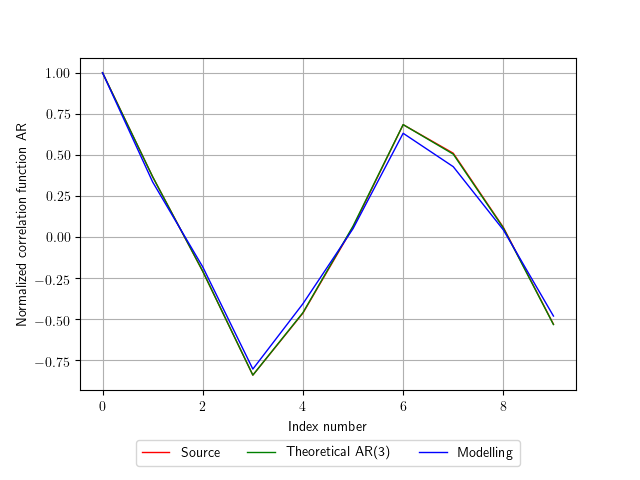
\includegraphics{plot_ar_ncf.png}
			\caption{Графическое сравнение НКФ для модели АР(3)}
		\end{figure}
		  	
		\begin{figure}[H]
			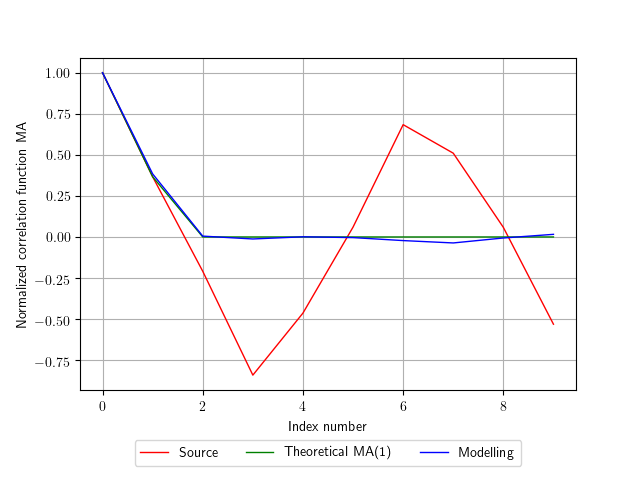
\includegraphics{plot_ma_ncf.png}
			\caption{Графическое сравнение НКФ для модели CC(1)}
		\end{figure}
		  	
		\begin{figure}[H]
			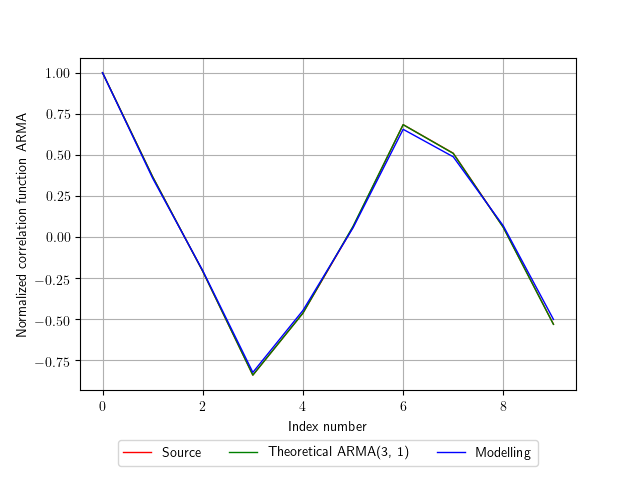
\includegraphics{plot_arma_ncf.png}
			\caption{Графическое сравнение НКФ для модели АРCC(3, 1)}
		\end{figure}
	} 
				
	%--------------------------------------------------
	% Итоговая таблица сравнения моделей АРСС
	%--------------------------------------------------
	\newpage
	\section{Итоговая таблица сравнения моделей АРСС}
	{
		В таблице 9 представлены итоговые результаты.
			  
		\begin{table}[H]
			\centering
			\caption{Итоговые результаты статистического анализа СП и моделирования}
			\begin{tabularx}{\textwidth}{ | >{\centering\arraybackslash}p{0.115\textwidth} | >{\centering\arraybackslash}p{0.1\textwidth} | >{\centering\arraybackslash}p{0.095\textwidth} | >{\centering\arraybackslash}p{0.095\textwidth} | Y | Y | >{\centering\arraybackslash}p{0.105\textwidth} | >{\centering\arraybackslash}p{0.105\textwidth} | }
				\hline
				Параметры процесса & Исходный процесс & АР(3) теория & АР(3) модель & СС(1) теория & СС(1) модель & АРСС(3,1) теория & АРСС(3,1) модель       \\ \hline
				Среднее                      & 99.95990                        & 99.95990             & 99.97495             & 99.95990             & 100.18219            & 99.95990                   & 99.96754 \tabularnewline \hline  
				Дисперсия                  & 248.5539                        & 248.5539             & 193.07658            & 248.5539             & 251.76423            & 248.5539                   & 208.87360 \tabularnewline \hline 
				СКО                              & 15.76559                        & 15.76559             & 13.89520             & 15.76559             & 15.86708             & 15.76559                   & 14.45246 \tabularnewline \hline  
				\multicolumn{8}{|c|}{Нормированная корреляционная функция} \tabularnewline \hline
				r(0)                                & 1.00000                         & 1.00000              & 1.00000              & 1.00000              & 1.00000              & 1.00000                    & 1.00000 \tabularnewline \hline   
				r(1)                                & 0.36654                         & 0.36654              & 0.32207              & 0.36654              & 0.37392              & 0.36654                    & 0.33774 \tabularnewline \hline   
				r(2)                                & -0.20896                        & -0.20896             & -0.17500             & 0.00000              & -0.00312             & -0.20896                   & -0.18725 \tabularnewline \hline  
				r(3)                                & -0.84118                        & -0.84118             & -0.80196             & 0.00000              & -0.00569             & -0.84118                   & -0.81092 \tabularnewline \hline  
				r(4)                                & -0.46353                        & -0.46067             & -0.38961             & 0.00000              & -0.00685             & -0.46353                   & -0.41711 \tabularnewline \hline  
				r(5)                                & 0.06005                         & 0.06634              & 0.04976              & 0.00000              & -0.00358             & 0.06523                    & 0.06031 \tabularnewline \hline   
				r(6)                                & 0.68374                         & 0.68406              & 0.62420              & 0.00000              & -0.00655             & 0.68365                    & 0.63791 \tabularnewline \hline   
				r(7)                                & 0.51005                         & 0.50414              & 0.41071              & 0.00000              & 0.00354              & 0.50863                    & 0.44453 \tabularnewline \hline   
				r(8)                                & 0.05844                         & 0.0545               & 0.05103              & 0.00000              & 0.01235              & 0.05715                    & 0.04911 \tabularnewline \hline   
				r(9)                                & -0.53115                        & -0.53334             & -0.46966             & 0.00000              & 0.00677              & -0.53210                   & -0.47669 \tabularnewline \hline  
				r(10)                               & -0.51157                        & -0.50832             & -0.39948             & 0.00000              & 0.00273              & -0.51341                   & -0.43103 \tabularnewline \hline  
				\multicolumn{2}{|c|}{Погрешность модели} & 0.00011 & 0.04005 & 2.24461 & 2.24212 & 0.00003 & 0.00349 \tabularnewline \hline
			\end{tabularx}
		\end{table}
					
		Для нахождения погрешности использовался критерий среднего квадратичного отклонения по первым десяти отсчётам:
		\begin{equation}
			\epsilon^2 = \sum_{k=1}^{10} {(r^{\text{М}}(k) - \hat{r}(k))^2},
		\end{equation}
	}
	где $\hat{r}(k)$ -- выборочная НКФ исходного процесса, $r^{\text{М}}$ -- выборочная НКФ смоделированного процесса.
				
	На рисунке 6 представлен смоделированный процесс АРСС(3, 1).
				
	\begin{figure}[H]
		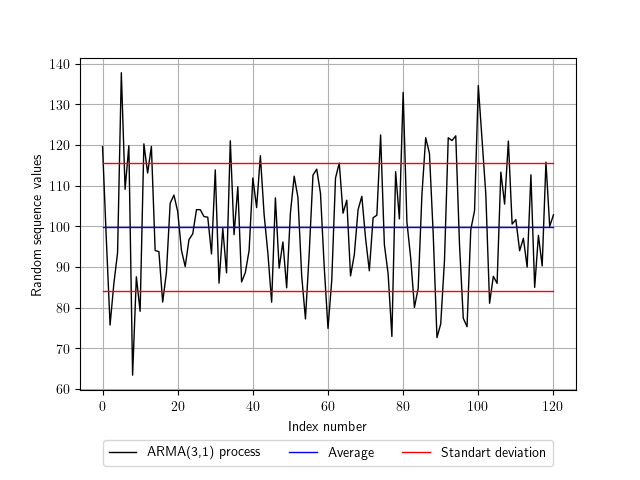
\includegraphics{plot_arma_modeled.png}
		\caption{Фрагмент реализации АРСС(3, 1)}
	\end{figure}
}
			
%--------------------------------------------------
% Заключение
%--------------------------------------------------
\newpage
\phantomsection
\addcontentsline{toc}{section}{Заключение}
\section*{Заключение}
{
	  	Задача моделирования случайных процессов является довольно частой и важной. Модели авторегрессии и скользящего среднего позволяют моделировать случайные процессы, подобные исходному, по уже имеющейся реализации.

	  	Было проведено исследование и моделирование для некоторого исходного неизвестного эргодического процесса. В ходе работы была проанализирована выборка из отсчётов исходного процесса, построены модели АР с помощью уравнений Юла-Уокера и модели СС с помощью систем нелинейных уравнений. Лучшими моделями в каждом классе оказались АР(3) и СС(1) с погрешностями 0.00011 и 2.24461 соответственно. Были построены смешанные модели АРСС до третьего порядка включительно, лучшей моделью среди них оказалась АРСС(3,1) с погрешностью равной 0.0001.
	  	
	  	Для каждой из трёх лучших моделей были смоделированы случайные процессы, рассчитаны выборочные моментные функции, а также был произведен сравнительный анализ построенных моделей. Наилучшей оказалась модель АРСС(3,1) с погрегостью равной 0.00349. 
}
			
%--------------------------------------------------
% Список литературы
%--------------------------------------------------
\newpage
\phantomsection
\addcontentsline{toc}{section}{Список литературы}
\section*{Список литературы}
{
	\begin{enumerate}
		\item {\textbf{Тараскин, А.Ф.} Статистический анализ временных рядов авторегрессии и скользящего среднего: учебное пособие [Текст] // Самара: СГАУ, 1998. – 56с.}
		\item {\textbf{Тараскин, А.Ф.} Статистическое моделирование и метод Монте–Карло: учебное пособие [Текст] // Самара: СГАУ, 1997. – 62с.}
		\item {\textbf{Храмов, А.Г.} Анализ и моделирование процессов АРСС: интернет-ресурс к курсовой работе [Электронный ресурс] // Самара: СГАУ, 2009.}
	\end{enumerate}
}
			
%----------------------------------------------------------------------------------------
			  
%------------------------------------------
% Приложения
%------------------------------------------
			  
			  
%------------------------------------------
% Текст программы
%------------------------------------------
\newpage
\phantomsection
\addcontentsline{toc}{section}{ПРИЛОЖЕНИЕ А Код программы}
\section*{ПРИЛОЖЕНИЕ А Код программы}
main.py:
\lstinputlisting[language=Python,mathescape=true]{./src/main.py}
			    
\newpage
correlation.py:
\lstinputlisting[language=Python,mathescape=true]{./src/correlation.py}
			    
\newpage 
moving\_average.py:
\lstinputlisting[language=Python,mathescape=true]{./src/moving_average.py}
				
\newpage
autoregression.py:
\lstinputlisting[language=Python,mathescape=true]{./src/autoregression.py}
				
\newpage 
arma.py:
\lstinputlisting[language=Python,mathescape=true]{./src/arma.py}
			
			
%--------------------------------------------------
% Метод простых итерации
%--------------------------------------------------
\newpage
\phantomsection
\addcontentsline{toc}{section}{ПРИЛОЖЕНИЕ Б Метод простых итераций}
\section*{ПРИЛОЖЕНИЕ Б Метод простых итерации}
{
	Итерационный метод решения системы нелинейных алгебраических уравнений рассмотрим на примере модели СС(2). Известно, что рассматриваемый ниже метод простых итераций для устойчивых моделей АРСС всегда позволяет найти одно из решений системы, если это решение существует. \medskip
		
	\textbf{Модель СС(2)}
	\begin{equation*}
		\eta_n = \alpha_0 \xi_n + \alpha_1 \xi_{n - 1} + \alpha_2 \xi_{n - 2}
	\end{equation*}
		
	Система нелинейных уравнений для расчёта $\alpha_0, \alpha_1, \alpha_2$ имеет вид:
	\begin{equation*}
		\left\{
		\begin{split}
			R_{\eta}(0) &= \alpha_0^2 + \alpha_1^2 + \alpha_2^2 \\
			R_{\eta}(1) &= \alpha_0 \alpha_1 + \alpha_1 \alpha_2 \\
			R_{\eta}(2) &= \alpha_0 \alpha_2
		\end{split}
		\right.
	\end{equation*}
						
	Значения $R_{\eta}(0), R_{\eta}(1), R_{\eta}(2)$ известны. \medskip
	  
	Начальное приближение: $\alpha_0 = \sqrt{R_{\eta}(0)}, \alpha_1 = 0, \alpha_2 = 0$. \medskip
	  
	Схема итераций:
	\begin{enumerate}
		\item {$\alpha_2 \leftarrow \displaystyle\frac{R_{\eta}(2)}{\alpha_0}$.}
		\item {$\alpha_1 \leftarrow \displaystyle\frac{R_{\eta}(1) - \alpha_1 \alpha_2}{\alpha_0}$.}
		\item {Если $R_{\eta}(0) < \alpha_1^2 + \alpha_2^2$, то решений нет, иначе $\alpha_0 \leftarrow \displaystyle\sqrt{R_{\eta}(0) - \alpha_1^2 - \alpha_2^2}$.}
		\item {Проверка на завершение итераций -- уменьшение скорости сходимости итераций до заданного значения $\epsilon$.}
		\item {Переход к пункту 1.}
	\end{enumerate}
	  
	В результате итерационного процесса будет найденно одно из возможных решений ситсемы, что является достаточным в данной работе, или же $R_{\eta}(0) < \alpha_1^2 + \alpha_2^2$, что говорит о том, что решений нет.
}
			
\end{document}
